\begin{figure}
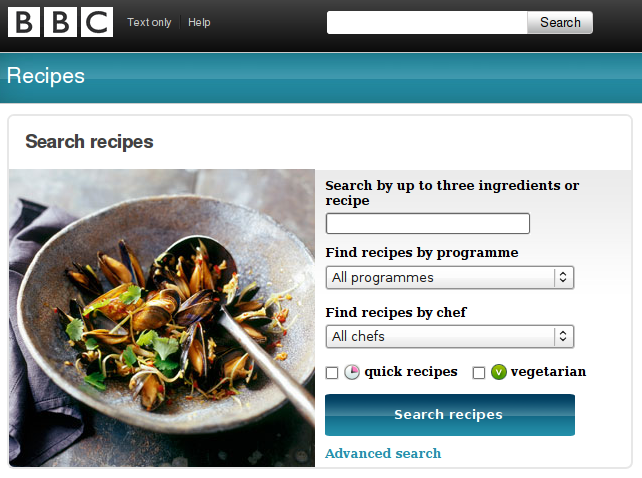
\includegraphics[width=0.9\textwidth]{screenshot_bbc_recipes}
\caption{The BBC Food Recipe Search Page}
\label{fig:bbc_food}
\end{figure}

The aim of this project is to develop a software kitchen assistant tool. This tool must be able to provide recipes which match a supplied list of available ingredients. This is similar to the BBC's recipe search\footnote{\url{http://www.bbc.co.uk/food/recipes/}} (Fig~\ref{fig:bbc_food}), but is not constrained to just three search items. The software should, in essence, provide recipe matches to help the user make recipe decisions given the ingredients he/she currently has. This involves making recommendations and provides us with an avenue to make use of collaborative filtering technology. Additionally, the recipe database can be community maintained, and aspects of social networking can be implemented to encourage user participation. The main draw of the project lies in its inherent flexibility, which extends from the plethora of expansion decisions which can be made to enhance user experience.
